\section{Variable elimination}

The factored representation of joint probability offers an efficient approach to marginalization by consolidating summations as deeply as feasible.
As we carry out these innermost summations, we generate fresh terms in the process.
\begin{example}
    In the Bayesian network depicted below:
    \begin{figure}[H]
        \centering
        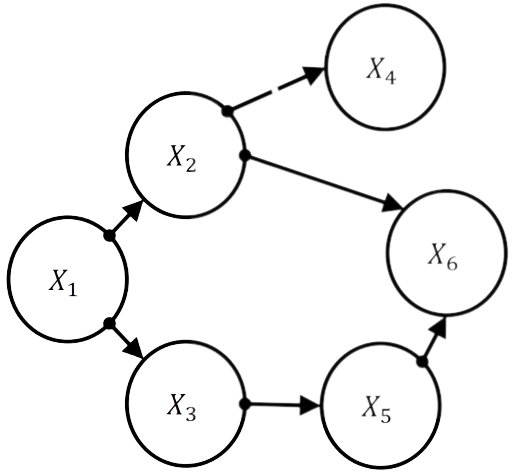
\includegraphics[width=0.25\linewidth]{images/bn.png}
    \end{figure}
    We can compute the probability distribution for $X_5$ as follows:
    \begin{align*}
        \textnormal{P}(X_5)     =& \sum_{X_1}\sum_{X_2}\sum_{X_3}\sum_{X_4}\sum_{X_6}\textnormal{P}(X_1)\textnormal{P}(X_2|X_1)\textnormal{P}(X_3|X_1)\textnormal{P}(X_4|X_2)\textnormal{P}(X_5|X_3)\textnormal{P}(X_6|X_5,X_2)          \\
                                =& \sum_{X_1}\sum_{X_2}\sum_{X_3}\sum_{X_6}\textnormal{P}(X_1)\textnormal{P}(X_2|X_1)\textnormal{P}(X_3|X_1)\textnormal{P}(X_5|X_3)\textnormal{P}(X_6|X_5,X_2)\sum_{X_4}\textnormal{P}(X_4|X_2)          \\ 
                                =& \sum_{X_1}\sum_{X_2}\sum_{X_3}\textnormal{P}(X_1)\textnormal{P}(X_2|X_1)\textnormal{P}(X_3|X_1)\textnormal{P}(X_5|X_3)\mu_1(X_2)\sum_{X_6}\textnormal{P}(X_6|X_5,X_2)\\
                                =& \sum_{X_2}\sum_{X_3}\textnormal{P}(X_5|X_3)\mu_1(X_2)\mu_2(X_5,X_2)\sum_{X_1}\textnormal{P}(X_1)\textnormal{P}(X_2|X_1)\textnormal{P}(X_3|X_1)     \\
                                =& \sum_{X_3}\textnormal{P}(X_5|X_3)\sum_{X_2}\mu_1(X_2)\mu_2(X_5,X_2)\mu_3(X_2,X_3)\\
                                =& \sum_{X_3}\textnormal{P}(X_5|X_3)\mu_4(X_3,X_5)\\
                                =& \mu_5(X_5)
    \end{align*}
\end{example}
The variable elimination procedure relies on dynamic programming. 
To utilize this approach, we break down the main problem into multiple smaller problems by leveraging the factorization of the joint distribution. 
This factorization not only guides us in establishing the most efficient order for variable elimination but also aids in determining the functions for the intermediate variables denoted as $\mu$.
To automate this procedure, we employ factor graph models, a type of graphical model wherein the box notation signifies terms dependent on specific variables. 
\begin{figure}[H]
    \centering
    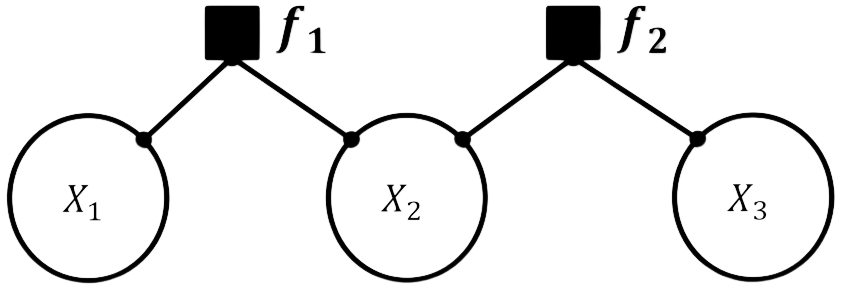
\includegraphics[width=0.25\linewidth]{images/fg.png}
    \caption{A simple example of a factor graph}
\end{figure}
The key characteristics of this graph include:
\begin{itemize}
    \item It constitutes a bipartite graph.
    \item Each circular node represents a random variable, denoted as $X_i$.
    \item Each boxed node represents a factor, labeled as $f_k$, which can be expressed as a function $f_k(X_{C_k})$. 
    \item The joint probability distribution is expressed as:
        \[\textnormal{P}(X_1,X_2,\dots,X_N)=\prod_{k=1}^K{f_k(X_{C_k})}\]
\end{itemize}
In this representation, the factor graph serves as a powerful tool for modeling and automating probabilistic calculations, offering a clear visual depiction of variable dependencies and factor relationships.

To convert a Bayesian network into a factor graph, the process involves applying a step called moralization. 
In the typical scenario, this operation entails establishing links between the parents of nodes while preserving as many independence properties as possible.
\begin{figure}[H]
    \centering
    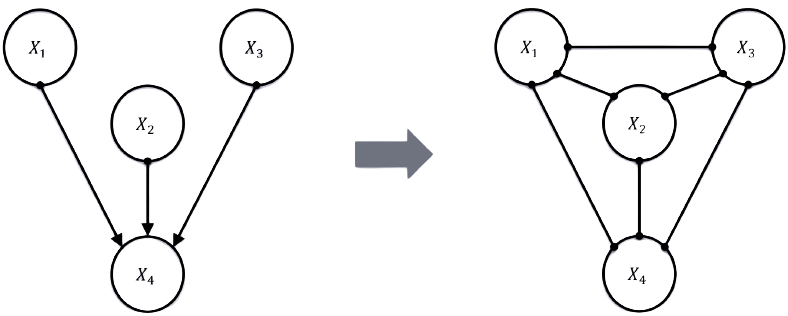
\includegraphics[width=0.5\linewidth]{images/mor.png}
    \caption{An example of moralization}
\end{figure}
To convert the Bayesian network into a factor graph, it's necessary to combine unconnected parents into a single factor.
\begin{example}
    In the provided Bayesian network:
    \begin{figure}[H]
        \centering
        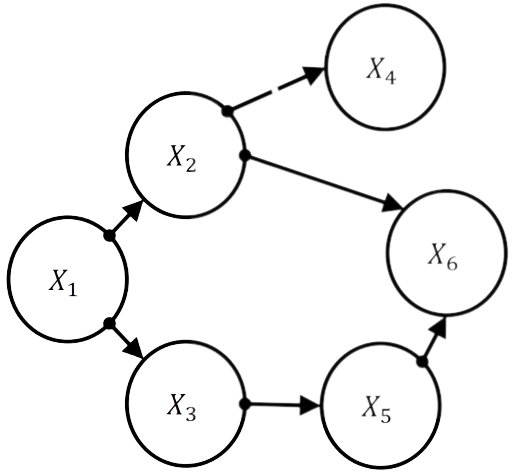
\includegraphics[width=0.25\linewidth]{images/bn.png}
    \end{figure}
    The corresponding factor graph is represented as follows:
    \begin{figure}[H]
        \centering
        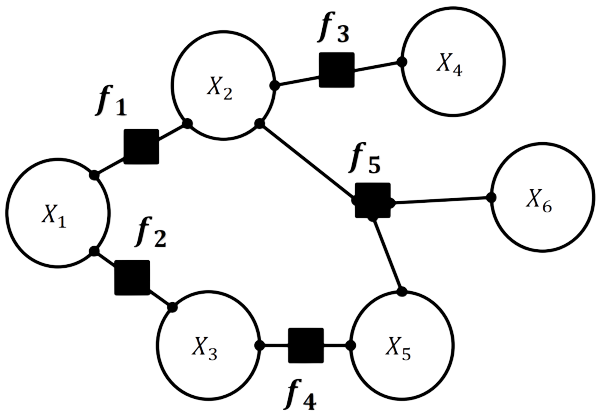
\includegraphics[width=0.25\linewidth]{images/bnf.png}
    \end{figure}
\end{example}
\begin{definition}
    A graph is a \emph{perfect map} if and only if every independence property of a distribution is reflected in the graph and vice versa. 
\end{definition}
Please be aware of the following:
\begin{itemize}
    \item Not all probability distributions can be faithfully depicted using directed or undirected graphs.
    \item Not all directed graphs can be transformed into undirected graphs while maintaining their original properties.
    \item Not all undirected graphs can be converted into directed graphs while preserving their original characteristics.
\end{itemize}
\begin{example}
    The chain can be portrayed as a factor graph in the following manner:
    \begin{figure}[H]
        \centering
        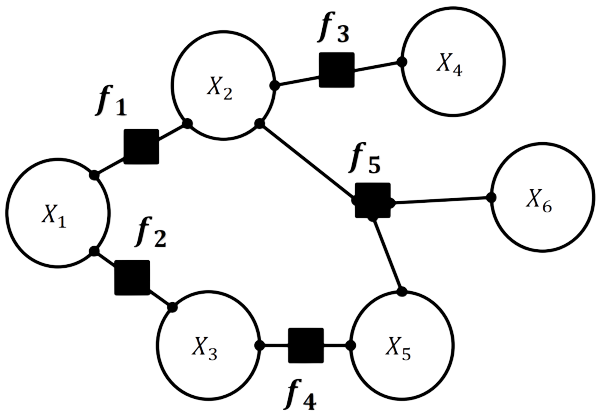
\includegraphics[width=0.3\linewidth]{images/bnf.png}
    \end{figure}
    \begin{itemize}
        \item $f_1(X_1)=P(X_1)$
        \item $f_2(X_1,X_2)=\textnormal{P}(X_1|X_2)$
        \item $f_3(X_2,X_3)=\textnormal{P}(X_3|X_2)$
        \item $f_4(X_3,X_4)=\textnormal{P}(X_4|X_3)$
        \item $f_5(X_4,X_5)=\textnormal{P}(X_5|X_4)$
        \item $f_5(X_5,X_6)=\textnormal{P}(X_6|X_5)$
    \end{itemize}
\end{example}
It's important to note that factor graphs are not unique; there are various ways to represent any given Bayesian network.

The variable elimination algorithm takes two inputs: a list denoted as $F$ containing factors and a tuple labeled as $C_0$ representing the output variables to retain. 
The result of the algorithm is a single factor $m$ that encompasses the variables in $X_{C_0}$.
\begin{algorithm}[H]
    \caption{Variable elimination algorithm}
        \begin{algorithmic}[1]
            \State define all variables present in $F$ as $V\leftarrow\textnormal{vars}(F)$
            \State define all variables to be eliminated as $E\leftarrow V-C_0$
            \For {all $i \in E$}
                \State call eliminate$\_$single$\_$variable$(F,i)$
            \EndFor
            \For {all remaining factors}
                \State $m \leftarrow \prod_{f \in F}f$
            \EndFor
        \end{algorithmic}
\end{algorithm}
The function eliminate$\_$single$\_$variable$(F,i)$ in the prior algorithm accepts as inputs the list of factors denoted as $F$ and the variable identified by $i$. 
It returns the updated list of factors, which remains labeled as $F$.
\begin{algorithm}[H]
    \caption{eliminate$\_$single$\_$variable$(F,i)$}
        \begin{algorithmic}[1]
            \State find relevant subset $f \subset F$ of factors over $i$ as $f \leftarrow\{C|i\in C\}$
            \State define the remaining clique as $C_t \leftarrow \textnormal{vars}(f)-\{i\}$
            \State compute the temporary factor as $\mu(X_{C_t})=\sum_{X_i}\prod_{f \in F}f$
            \State remove old factors $f$ and append new temporary factor $t$ to $F$
            \State \Return $F$
        \end{algorithmic}
\end{algorithm}
\begin{example}
    Consider the Bayesian network illustrated below:
    \begin{figure}[H]
        \centering
        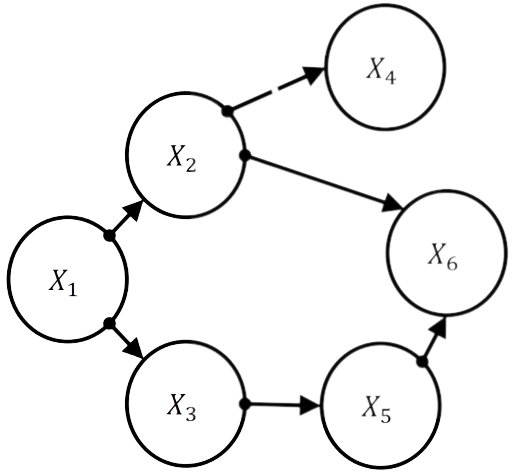
\includegraphics[width=0.25\linewidth]{images/bn.png}
    \end{figure}
    We can compute the factor graph with moralization, resulting in the following factor graph:
    \begin{figure}[H]
        \centering
        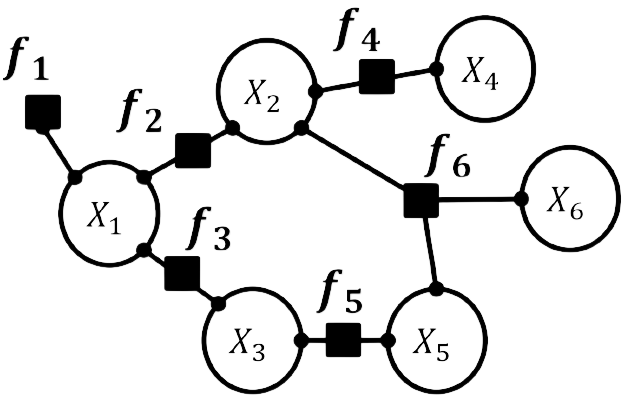
\includegraphics[width=0.25\linewidth]{images/bnf1.png}
    \end{figure}
    Now, let's compute the marginal probability $\textnormal{P}(X_1,X_6)=\mu(X_1,X_6)$. To do this, we'll utilize the variable elimination algorithm with the following inputs:
    \begin{itemize}
        \item $F=\{f_1,f_2,f_3,f_4,f_5,f_6\}$
        \item $C_0=\{X_1,X_6\}$
    \end{itemize}
    The algorithm progresses as follows:
    \begin{enumerate}
        \item Define all the variables present in $F$: 
            \[V=\{X_1,X_2,X_3,X_4,X_5,X_6\}\]
        \item Calculate the set of variables to be eliminated:
            \[E=V-C_0=\{X_1,X_2,X_3,X_4,X_5,X_6\}-\{X_1,X_6\}=\{X_2,X_3,X_4,X_5\}\]
    \end{enumerate}
    Now, we need to eliminate the single variables contained in set $E$ using the  eliminate$\_$single$\_$variable function. Here's the step-by-step process for each variable:
    \begin{itemize}
        \item Eliminate $X_4$: 
            \begin{itemize}
                \item Check the connected functions: $f=\{f_4\}$. 
                \item The clique containing $X_4$ (excluding itself) is: $C_t=\{X_2\}$. 
                \item Calculate the temporary factor: $\mu_1(X_2)=\sum_{X_4}P(X_4|X_2)$. 
                \item Update $F$ to: $F=\{f_1,f_2,f_3,f_5,f_6,\mu_1\}$. 
                \item Remove $f$ from $E$, resulting in $E=\{X_2,X_3,X_5\}$
            \end{itemize}
        \item Eliminate $X_3$: 
            \begin{itemize}
                \item Check the connected functions: $f=\{f_3,f_5\}$. 
                \item The clique containing $X_3$ (excluding itself) is: $C_t=\{X_1,X_5\}$. 
                \item Calculate the temporary factor: $\mu_2(X_1,X_5)=\sum_{X_3}P(X_3|X_1)P(X_5|X_3)$. 
                \item Update $F$ to: $F=\{f_1,f_2,f_6,\mu_1,\mu_2\}$. 
                \item Remove $f$ from $E$, resulting in $E=\{X_2,X_5\}$
            \end{itemize}
        \item Eliminate $X_5$: 
            \begin{itemize}
                \item Check the connected functions: $f=\{f_6,\mu_2\}$. 
                \item The clique containing $X_5$ (excluding itself) is: $C_t=\{X_1,X_2,X_6\}$. 
                \item Calculate the temporary factor: $\mu_3(X_1,X_2,X_6)=\sum_{X_5}\mu_2(X_1,X_5)P(X_6|X_2,X_5)$. 
                \item Update $F$ to: $F=\{f_1,f_2,\mu_1,\mu_3\}$. 
                \item Remove $f$ from $E$, resulting in $E=\{X_2\}$
            \end{itemize}
        \item Eliminate $X_2$: 
            \begin{itemize}
                \item Check the connected functions: $f=\{f_2,\mu_1,\mu_3\}$. 
                \item The clique containing $X_2$ (excluding itself) is: $C_t=\{X_1,X_6\}$. 
                \item Calculate the temporary factor: $\mu_4(X_1,X_6)=\sum_{X_2}\mu_1(X_2)P(X_2|X_1)\mu_3(X_1,X_2,X_6)$. 
                \item Update $F$ to: $F=\{f_1,\mu_4\}$. 
                \item Remove $f$ from $E$, resulting in $E=\varnothing$
            \end{itemize}
    \end{itemize}
    After these iterations, we have the following results:
    \begin{itemize}
        \item $F=\{f_1,\mu_4\}$
        \item $C_0=\{X_1,X_6\}$
    \end{itemize}
    The final steps involve multiplying all the elements in $f$: 
    \[\textnormal{P}(X_1,X_6)=\mu_4 \cdot f_1=P(X_1)\mu_4(X_1,X_6)\]
    This yields the marginal probability $\textnormal{P}(X_1,X_6)$ using the variable elimination algorithm.
\end{example}
It's worth mentioning that the order in which variables are selected as input for the function can be determined using a heuristic function. 
One common approach is to order the nodes based on the ascending number of connections they have in the factor graph.
\begin{example}
    Given the Bayesian network and the associated truth tables:
    \begin{figure}[H]
        \centering
        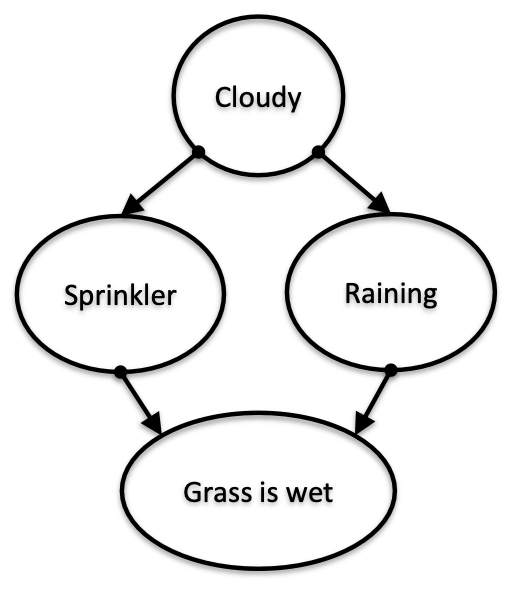
\includegraphics[width=0.3\linewidth]{images/sprinkler.png}
    \end{figure}
    \begin{table}[H]
        \centering
        \begin{tabular}{cc}
        \hline
        \textbf{Cloudy} & \textbf{P(C)} \\ \hline
        0      & 0.5  \\
        1      & 0.5  \\ \hline
        \end{tabular}
    \end{table}
    \begin{table}[H]
        \centering
        \begin{tabular}{ccc}
        \hline
        \textbf{Sprinkler} & \textbf{Cloudy} & \textbf{P(S$|$C)} \\ \hline
        0         & 0      & 0.1  \\
        0         & 1      & 0.5  \\
        1         & 0      & 0.9  \\
        1         & 1      & 0.5  \\ \hline
        \end{tabular}
    \end{table}
    \begin{table}[H]
        \centering
        \begin{tabular}{ccc}
        \hline
        \textbf{Raining} & \textbf{Cloudy} & \textbf{P(R$|$C)} \\ \hline
        0       & 0      & 0.8    \\
        0       & 1      & 0.5    \\
        1       & 0      & 0.2    \\
        1       & 1      & 0.5    \\ \hline
        \end{tabular}
    \end{table}
    \begin{table}[H]
        \centering
        \begin{tabular}{cccc}
        \hline
        \textbf{Wet} & \textbf{Sprinkler} & \textbf{Raining} & \textbf{P(W$|$S,R)} \\ \hline
        0            & 0                  & 0                & 1                   \\
        0            & 0                  & 1                & 0.1                 \\
        0            & 1                  & 0                & 0.1                 \\
        0            & 1                  & 1                & 1                   \\
        1            & 0                  & 0                & 0                   \\
        1            & 0                  & 1                & 0.9                 \\
        1            & 1                  & 0                & 0.9                 \\
        1            & 1                  & 1                & 0.99                \\ \hline
        \end{tabular}
    \end{table}
    We want to compute $\textnormal{P}(W)$. To do this, we start by transforming the Bayesian network into a factor graph, where we define the factors as follows:
    \begin{itemize}
        \item $f_1(C)=\textnormal{P}(C)$.
        \item $f_2(S,C)=\textnormal{P}(S|C)$.
        \item $f_3(R,C)=\textnormal{P}(R|C)$.
        \item $f_4(W,S,R)=\textnormal{P}(W|S,R)$.
    \end{itemize}
    The resulting factor graph looks like this:
    \begin{figure}[H]
        \centering
        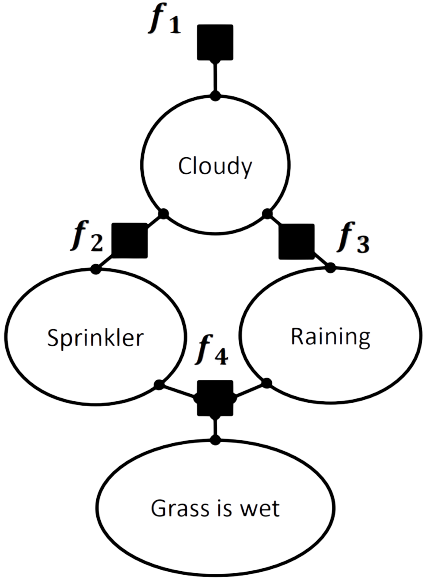
\includegraphics[width=0.25\linewidth]{images/sprinklerfg.png}
    \end{figure} 
    After applying the variable elimination algorithm, we obtain the following graph:
    \begin{figure}[H]
        \centering
        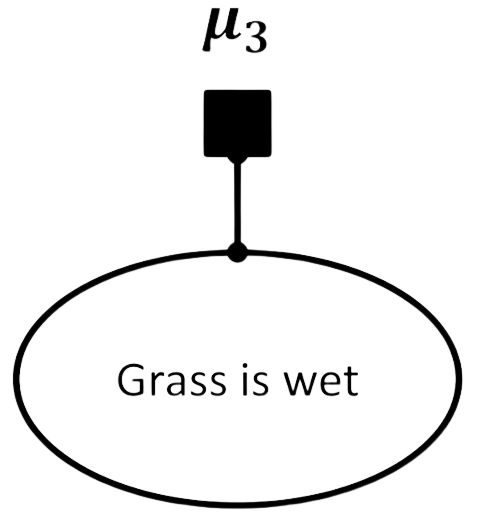
\includegraphics[width=0.15\linewidth]{images/fg1.png}
    \end{figure} 
    The corresponding truth table for the variable $\mu_3(W)$ is as follows:
    \begin{table}[H]
        \centering
        \begin{tabular}{cc}
        \hline
        \textbf{Wet} & \textbf{$\boldsymbol{\mu_3}$(W)} \\ \hline
        0      & 0.22915  \\
        1      & 0.77085  \\ \hline
        \end{tabular}
    \end{table}
\end{example}
Variable elimination possesses several advantages, including its simplicity of implementation and the faithful representation of manual calculations. 
With an optimal ordering, its complexity is $O(N2^K)$.
However, it does have its drawbacks. 
Finding the optimal ordering is an $\mathcal{NP}$-hard problem, it can compute only one marginal at a time, and computing all marginals necessitates $N$ executions, which can be inefficient for more extensive networks.